\chapter{Calibrating and Characterizing Controlled Arbitrary Phase Gates} \label{ch:carb}
\glsreset{carb}
This chapter details the concepts, calibration and characterization of \glspl{carb}. We start by explaining how this gate family can be seen as an extension of standard conditional phase gate (\glspl{cz}). Next, we demonstrate the implementation of a \gls{carb}, allowing us to reach continuous conditional phase in the range $[0, 2\pi[$. We describe the calibration procedure of the gate on qubit 2 and 3 of our quantum processor presented in Appendix~\ref{app:setup}. Next, perform quantum process tomography and evaluate the process fidelity as a function of conditional phase. By exploiting the 3-level readout discussed in Appendix~\ref{ch:qutrit_readout}, we then characterize conditional- and dynamic phase errors and leakage. We compare these phase errors and leakage values to the ones obtained with a \gls{cz} implemented on the same qubits.

\section{Theoretical description} \label{sec:c_arb_theory}
In this section, we derive the unitary evolution of the \gls{carb} and explain the physical mechanisms behind its implementation. The goal is to obtain a unitary operator $U_{\textrm{C-ARB}}$ in a two-qubit subspace which adds a controllable phase $\phi$ to the \oo{} state, 
\begin{equation} \label{eq:carb_unitary}
    U_{\textrm{C-ARB}}=
    \begin{pmatrix}
{1} & {0} & {0} & {0} \\
{0} & {1} & {0} & {0} \\
{0} & {0} & {1} & {0} \\
{0} & {0} & {0} & {e^{-\i \phi}}
\end{pmatrix}
\end{equation}

We obtain such unitary by exploiting the same effect as for the \gls{cz}, namely the collection of geometric phase on the \oo{} state due to the interaction of the \oo{} level and the non-computational \tz{} level~\cite{Strauch2003QuantumQubits, DiCarlo2009DemonstrationProcessor}. As pictured in Fig.~\ref{fig:carb_theory}(a),  the \oo{} and \tz{} levels hybridize strongly when they are brought close to resonance. In this regime, we can approximate their interaction as a two-level system where the ground (excited) state is the \oo{} (\tz{}) state. The system is characterized by the Hamiltonian
\begin{equation}
    \hat H/\hbar= \omega_{\ket{11}} \oo{} \bra{11} + \omega_{\ket{20}} \tz{} \bra{20} + J( \oo{}\bra{20}+ \tz{}\bra{11})
\end{equation}
where  $\omega_{\ket{11}}$ ($\omega_{\ket{20}}$) is the frequency of the energy level \oo{} (\tz{}), and $J$ is the fixed coupling strength between the two levels which is a chip design parameter fixed during fabrication. The first and second term in the Hamiltonian correspond to the energy in the \oo{} and \tz{} level respectively. The third term represents the coupling energy between the two levels in which the excitation is transferred from one level to the other and vice-versa. 

The same Hamiltonian can conveniently be written in matrix form with basis vectors \oo{} and \tz{},
\begin{equation}
\hat{H}/\hbar=
\begin{pmatrix}
\omega_{\oo} & J \\
J & \omega_{\tz}
\end{pmatrix}
\end{equation}
We shift the zero energy to $\omega_{\oo}$  and define the frequency detuning between the two levels $\Delta = \omega_{\tz}- \omega_{\oo}$ such that $\hat H$ becomes
\begin{equation}
\hat{H}/\hbar=
\begin{pmatrix}
0 & J \\
J & \Delta
\end{pmatrix}
\end{equation}

From Schr\"odinger's equation, it follows that the time evolution of an arbitrary state $\ket{\psi}$ in the \oo-\tz{} subspace is given by $|\psi(t)\rangle = U(t)\ket{\psi}$ where $U(t) = \sexp{-\i \hat H/\hbar t}$ is the unitary evolution of the Hamiltonian. Specifically, the unitary $U(t)$ is defined as,
\begin{equation}
\begin{split}
    &U(t) = \\
& \begin{pmatrix}
 \sexp{-\frac{1}{2} \i t \Delta } \left(\cos \left(\frac{1}{2} t \Tilde{J} \right)+\frac{\i \Delta  \sin \left(\frac{1}{2} t \Tilde{J}\right)}{\Tilde{J}}\right) & -\frac{2 \i e^{-\frac{1}{2} \i t
   \Delta } J \sin \left(\frac{1}{2} t \Tilde{J}\right)}{\Tilde{J}} \\
 -\frac{2 \i e^{-\frac{1}{2} \i t \Delta } J \sin \left(\frac{1}{2} t \Tilde{J}\right)}{\Tilde{J}} & \sexp{-\frac{1}{2} \i t \Delta }
   \left(\cos \left(\frac{1}{2} t \Tilde{J}\right)-\frac{\i \Delta 
   \sin \left(\frac{1}{2} t \Tilde{J}\right)}{\Tilde{J}}\right) \\
\end{pmatrix}
\end{split}
\end{equation}
where we have defined for clarity $\Tilde{J} := \sqrt{4J^2+\Delta^2}$ which we call the \textit{effective exchange coupling}.

When starting with an excitation in the \oo{} state (the ground-state of this two-level subsystem), the \oo{} population oscillates coherently as the excitation is swapped back and forth between the \oo{} and the \tz{} state,
\begin{equation}
P_{\oo{}}(t) = \mathrm{Tr}\left(U(t)\ket{11}\bra{11}U^\dag(t)\right) = \frac{\Delta ^2+2 J^2 (\cos \left(t \sqrt{4J^2+\Delta^2}\right)+1)}{4J^2+\Delta^2}
\end{equation}
with an oscillation period of $2\pi/\Tilde{J}$. 

The population as function of frequency detuning $\Delta$ and interaction time $t$ results in a Chevron pattern shown in Fig.~\ref{fig:carb_theory}(b). For the operating point of the \gls{cz}, $\Delta = 0$, the population is given by $P_{\oo{}} = \frac{1}{2} + \frac{1}{2}\cos{2Jt}$. This corresponds to a complete population exchange between the \oo{} and the \tz{} state and with an oscillation period of $\pi/J$. By contrast, $\Delta \neq 0$ results in a partial population exchange between the \oo{} and the \tz{} state. The oscillation period is also reduced due to the detuning $\Delta$ in the denominator. 

\begin{figure}
    \centering
    \includegraphics[width=1\textwidth]{chapters/carb_gate/figs/ch4_carb_theory_c3_20200312_095516.png}
    \caption{Simulation of the \gls{carb} as a generalization of the \gls{cz}. (a) Avoided crossing between the \oo{} (brown) and the \tz{} (orange) energy levels as function of detuning. (b) Population of the \oo{} state as function of frequency detuning $\Delta$ and interaction time $t$ (in units of $J$) visualizing the coherent population exchange due to hybridization. The dashed line corresponds to the frequency detunings and gate lengths resulting in the first maximum in population recovery in the computational subspace. (c) Conditional phase acquired on the \oo{} state resulting from the interaction of the two levels. We reach all conditional phases between 0 and $2\pi$ by sweeping the detuning and adapting the time accordingly to ensure population recovery (dashed line). }
    \label{fig:carb_theory}
\end{figure}

The gate length must be an integer multiple of the oscillation period to ensure a unitary operation within the computational subspace (i.e.\ full population recovery). In Fig.~\ref{fig:carb_theory}(b), we highlight (dashed line) the first oscillation period which corresponds to the shortest possible gate length as a function of the frequency detuning,
\begin{equation} \label{eq:carb_t_gate}
    t_{\textrm{C-ARB}} = \frac{2\pi}{\sqrt{4J^2+\Delta^2}}
\end{equation}

In  Fig.~\ref{fig:carb_theory}(c),  we illustrate the acquired conditional phase, $\phi$, as a function of detuning and gate length. For the gate lengths $t_{\textrm{C-ARB}}$, the corresponding phase on the \oo{} state acquired by the closed loop state evolution is
 \begin{equation} \label{eq:ch4_acquired_cond_phase}
     \phi = \mathrm{Arg}\Big(\bra{11}U(t_{\textrm{C-ARB}})\oo\Big) =  \pi \cdot \left( 1 + \frac { \Delta } { \sqrt { \Delta ^ { 2 } + 4 J ^ { 2 } } } \right)
 \end{equation}
which spans the interval $[0, 2\pi[$ for a sufficiently large detuning sweep, see dashed line in Fig.~\ref{fig:carb_theory}(c). As expected, a zero detuning yields a conditional phase of $\pi$ and therefore corresponds to the standard \gls{cz}.

In practice, we achieve these timed interactions with flux pulses\footnote{In fact, we apply a \textit{voltage} pulse at the output of the \gls{awg} and the latter creates a current in the flux line which results in magnetic flux through the SQUID loop} which shift the transition frequency of the individual qubits. For a gate in the off-state, we ensure $|\Delta|\gg J$ such that the acquired conditional phase is small. Ideally, the acquired phase should be zero but in practice it is not due to the residual $ZZ$-coupling between the \oo{} and the \tz{} state. To turn on the gate, we apply a square flux pulse with amplitude $a$ and length $l$ to one of the qubits via its flux line. The pulse shifts the \oo{} state non-adiabatically close to the \tz{} state. 

As mentioned in Section~\ref{sec:intro_building_qc}, the flux affects the Josephson energy~\cite[Eq.~2.18]{KochCharge-insensitiveBox}, 
\begin{equation}\
    E_J(a) = E _ { J , \max } \sqrt { \cos ^ { 2 } \left( \frac{\pi}{\Phi_0} \frac { \partial \Phi } { \partial V } a \right) + d ^ { 2 } \sin ^ { 2 } \left( \frac{\pi}{\Phi_0}\frac { \partial \Phi} { \partial V } a \right) }
\end{equation}
where $d$ is the asymmetry between the junctions in the SQUID loop of the transmon, $ \partial \Phi /\partial V $ is the flux sensitivity (voltage to flux conversion parameter), $\Phi_0 = h/2e$ is the superconducting flux quantum and $E _ { J , \max }$ is the maximal junction energy. 

In turn, the Josephson energy shifts the qubit transition frequency as defined by Eq.~\eqref{eq:qubit_frequency} such that
\begin{equation} \label{eq:carb_theory_freq01}
    \omega_{|01\rangle}(a) \simeq \sqrt{8  E _ { J , \max } \sqrt { \cos ^ { 2 } \left( \frac{\pi}{\Phi_0}\frac { \partial \Phi } {  \partial V } a \right) + d ^ { 2 } \sin ^ { 2 } \left( \frac{\pi}{\Phi_0}\frac { \partial \Phi} { \partial V } a \right)} E_{C}}-E_{C} 
\end{equation}
where we approximate $|E_c|$ to be equal to the anharmonicity $|\alpha_2|$ of the fluxed transmon~\cite[Eq. 2.12]{KochCharge-insensitiveBox}. 
The frequency detuning, $\Delta$, as function of the flux pulse amplitude is then simply
 \begin{equation}\label{eq:carb_detuning}
\begin{aligned} 
\Delta(a) & = \omega _ { | 20 \rangle } - \omega _ { | 11 \rangle } \\ 
& = 2 \omega _ { | 10 \rangle } - \alpha _ { 1 } - \left( \omega _ { | 10 \rangle } + \omega _ { | 01 \rangle }(a) \right) \\ 
& = \omega _ { | 10 \rangle } - \alpha _ { 1 } - \omega _ { | 01 \rangle }(a) 
\end{aligned}
\end{equation}
where $\alpha_1$ is the anharmonicity of the  transmon which is not fluxed.

It follows that varying the amplitude of the flux pulse indeed controls the frequency detuning between the \oo{} and the \tz{} state, which in turn controls the collected phase on the \oo{} state. To ensure full population recovery in the computational subspace, the length of the flux pulse must be $t_{\textrm{C-ARB}}$ which can be related back to the amplitude of the flux pulse by combining Eq.~\eqref{eq:carb_t_gate}, \eqref{eq:carb_theory_freq01} and \eqref{eq:carb_detuning},
\begin{equation} \label{eq:carb_t_gate_from_ampl}
\begin{split}
    &t_{\textrm{C-ARB}}(a)\simeq\\
    &   \frac{2\pi}{\sqrt{4J^2+\left(\omega _ { | 10 \rangle } - \alpha _ { 1 } - \sqrt{8  E _ { J , \max } \sqrt { \cos ^ { 2 } \left( \frac{\pi}{\Phi_0}\frac { \partial \Phi } {  \partial V } a \right) + d ^ { 2 } \sin ^ { 2 } \left( \frac{\pi}{\Phi_0}\frac { \partial \Phi} { \partial V } a \right)} \alpha_2} - \alpha_2 \right)^2}}
\end{split}
\end{equation}
In Section~\ref{sec:carb_calibration}, we fit Eq.~\eqref{eq:carb_t_gate_from_ampl} to experimental data to estimate $J$, $ \partial \Phi/ \partial V $ and $d$ and thereby also the expected conditional phase using Eq.~\eqref{eq:ch4_acquired_cond_phase}.

In addition to the conditional phase, the flux pulse also results in a dynamic phase $\phi_D$ on the fluxed qubit,  because it takes the qubit out of its rotating frame~\cite{DiCarlo2009DemonstrationProcessor},
\begin{equation} \label{eq:carb_dyn_phase}
    \phi_D = \int_0^l{(\omega(t)-\omega_{\textrm{park}})\d t}
\end{equation}
where $\omega(t)$ and $\omega_{\textrm{park}}$ denote the instantaneous qubit frequency during the pulse and the frequency at parking position\footnote{The parking position refers to the frequency of the qubit when the gate is off. We typically choose it to be where the derivative of the frequency with respect to flux is 0 to minimize the charge noise, a point we call the "sweet spot"~\cite{Vion2003QuantumProcessing}}, respectively. We compensate for this single-qubit phase shift with a virtual $Z$ gate after the \gls{carb}.

While the \gls{cz} is composed of from a single detuning and gate length, the \gls{carb} requires a careful interpolation of distinct detunings and corresponding gate lengths to span all possible conditional phases with high \oo{} population recovery. In addition, since the qubit frequency excursion depends on $\Delta$, dynamic phases have to be calibrated for all possible detuning/gate-length pairs. We detail the calibration procedure of these three continuous parameters in the next section.

\section{Calibration} \label{sec:carb_calibration}
This section describes the calibration procedure of a \gls{carb} using a square flux pulse on qubit 2 and 3 of the device presented in Appendix~\ref{app:setup}. To account for the finite rise-time and ensure a stable voltage at the output of the \gls{awg}, we filter the square pulse with a 1\unit{ns} Gaussian kernel. The calibration of the \gls{carb} consists of three measurements, illustrated in Fig.~\ref{fig:ch4_calibration_carb}.

First, we calibrate the pulse lengths to ensure maximum population recovery. We prepare the \oo{} state and perform a two-dimensional sweep of the flux pulse amplitude and length. For each amplitude and length, we measure the \1{} population of qubit 2 after the flux pulse using 3-level readout, yielding the Chevron pattern shown in Fig.~\ref{fig:ch4_calibration_carb}(a). Brighter areas correspond to high
level population of qubit 2, indicating the population is fully swapped back from the \2{} level into the computational subspace. To find the pulse lengths corresponding to the first period of the population exchange, we fit the \1{} population oscillation to a cosine for each pulse amplitude of the two-dimensional sweep. We then retrieve the pulse length corresponding to the first maximum of the population recovery.

We fit the pulse lengths corresponding the maximum population recovery to Eq.~\eqref{eq:carb_t_gate_from_ampl} to extract the flux sensitivity $\frac { \partial \Phi} { \partial V }$, the asymmetry between the junctions in the SQUID loop $d$  and the coupling strength $J$ between the \oo{} and \tz{} states. The fit is shown as a dashed line in Fig.~\ref{fig:ch4_calibration_carb}(a). We obtain a flux sensitivity of $\frac { \partial \Phi} { \partial V } / \Phi_0 = 0.34 \pm 0.01 \unit{\frac{1}{V}}$, an asymmetry of $0.7884 \pm 0.0003$ and a coupling of $J/2\pi =  4.72 \pm 0.05 \unit{MHz}$, all of which are consistent with previous characterization of this device~\cite{Andersen2019, Andersen2019a}.

Next, we measure the conditional phase as function of flux pulse amplitudes (see Fig.~\ref{fig:ch4_calibration_carb}(b)) while adapting the pulse length to maximize population recovery (see Fig.~\ref{fig:ch4_calibration_carb}(a), black circles). If necessary, pulse length is interpolated linearly between the calibration points of the pulse length calibration. The colored flux pulses shown in the pulse scheme in Fig.~\ref{fig:ch4_calibration_carb}(e) correspond to the diamond-shaped data points of respective color in ~\ref{fig:ch4_calibration_carb}(b). Using the parameter values obtained from the fit in Fig.~\ref{fig:ch4_calibration_carb}(a), we compute the expected conditional phase from  Eq.~\eqref{eq:ch4_acquired_cond_phase} and plot it in dashed line in Fig.~\ref{fig:ch4_calibration_carb}(b). The measured conditional phase saturates at a value of different than 0 due the phase acquired via the a residual $ZZ$-coupling of $\alpha_{ZZ} = 400\unit{kHz}$ over the period the pulse length and buffers (25ns) that separates the two $R_x^{\pi/2}$-pulses. 

Finally, we measure the dynamic phase the fluxed qubit acquires during its frequency excursion (see Fig.~\ref{fig:ch4_calibration_carb}(c)) with the pulse scheme presented in Fig.~\ref{fig:ch4_calibration_carb}(f)). With the approximation that its frequency is constant over the entire pulse at the value given by Eq.~\eqref{eq:carb_theory_freq01}, we compute the expected dynamic phase from Eq.~\eqref{eq:carb_dyn_phase} and show it with a dashed line. This measurement requires a high number of calibration points, as the dynamic phase grows rapidly as a function of detuning yet can only be measured in the $[0, 2\pi[$ interval (a minimum of 3 points per $[0, 2\pi[$ interval are required to ensure correct unwrapping). In Fig.~\ref{fig:ch4_calibration_carb}(c), only one out of three points is shown for clarity. 
\begin{figure}[H]
    \centering
    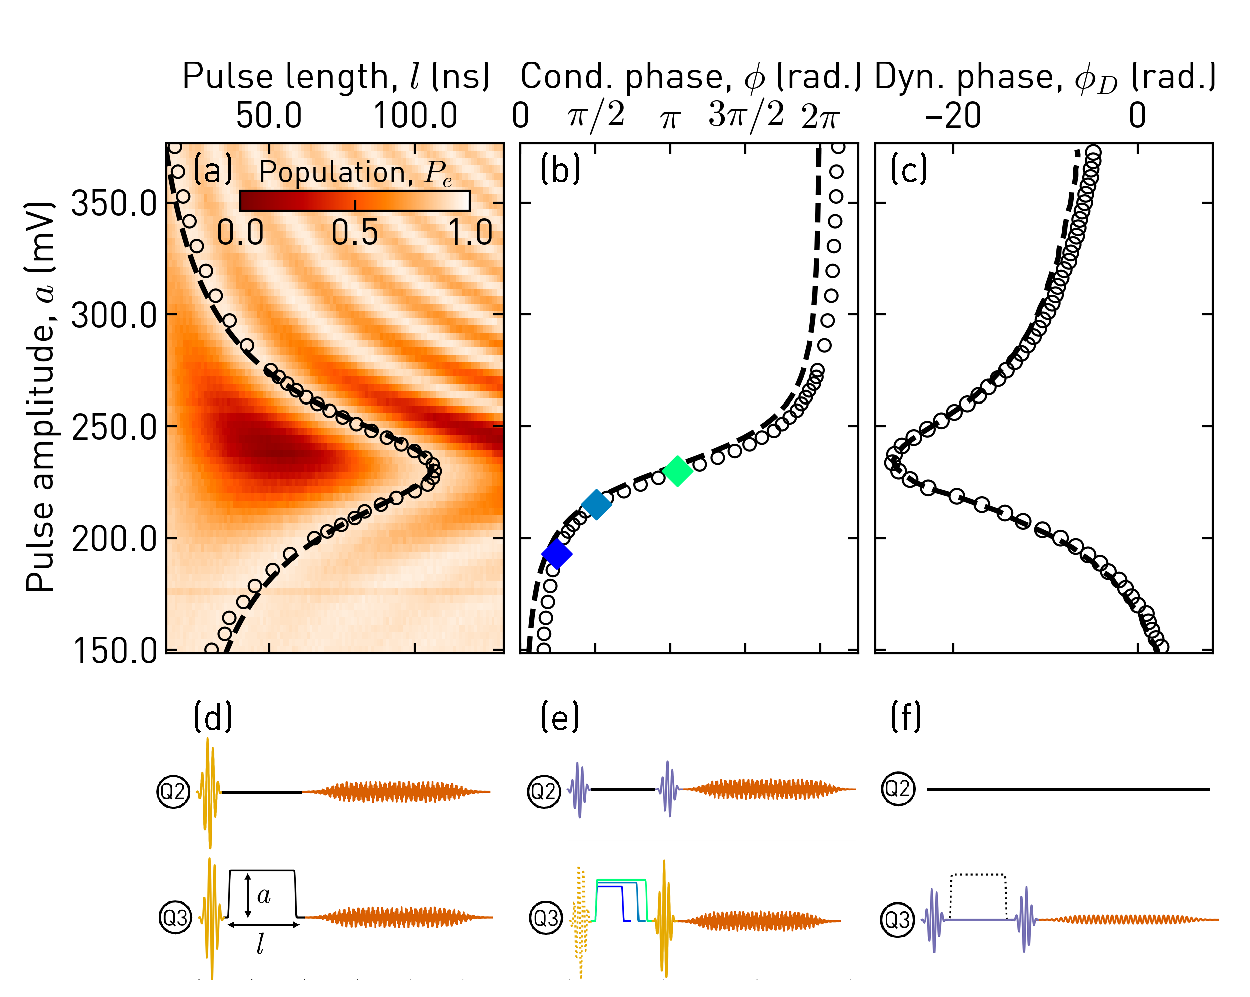
\includegraphics[width=\textwidth]{chapters/carb_gate/figs/ch4_carb_calibration_20200406_215519.pdf}
    \caption{Three calibration measurements (a, b, c) of a \gls{carb} and their corresponding pulse schemes (d, e, f).  (a) Qubit 2 \e{} level population as function of the flux pulse amplitude and length. The inset details the pulse scheme: the \oo{} state is prepared, the flux pluse (black) is  applied to qubit 3, the two qubits are read out with a multiplexed readout pulse. The scattered points correspond to the amplitudes and lengths used to calibrate the conditional phase (see b). The dashed line corresponds to the fit to the theoretical model. (b) Conditional phase as function of flux pulse amplitude. The amplitude sampling is not uniform to account for the non-linearity of the conditional phase. The dashed line indicates the phase predicted of the model (see main text for details).  (c) Unwrapped dynamic phase of qubit 3 as function of pulse amplitude. Only one out of three data point is shown for clarity.  The dashed line corresponds to the dynamic phase predicted by theory (see main text for details). (d) Pulse scheme corresponding to the two-dimensional parameter sweep shown in (a). The \oo{} state is prepared with two single-qubit $R_x^\pi$ (yellow), followed by the flux pulse (black) of amplitude $a$ and length $l$, and finally a readout pulse (orange). (e) Pulse scheme to measure conditional phase (see b). The phase is measured on qubit 2 with a Ramsey experiment (two $R_x^{\pi/2}$ pulses (purple)), while qubit 3 is fluxed once with and once without preceding single-qubit $R_x^{\pi}$ (dashed yellow). The difference between the two measurements yields the conditional phase. The different flux pulse colors result in the conditional phases indicated with diamonds of corresponding color in (b). (f) The dynamic phase is measured by comparing the phase of the qubit via a Ramsey experiment with and without flux pulse (dashed black).}
    \label{fig:ch4_calibration_carb}
\end{figure}

Due to flux cross-talk between the flux lines, the qubit staying at its parking position also acquires a non-zero dynamic phase. However, the latter is not calibrated, as flux cross-talk between the flux line of qubit 1 (3) and qubit 2 is smaller than 2\% (3\%) for the two two-qubit gates considered in this report~\cite{Andersen2018SampleB4QP3}.

The calibration time of the \gls{carb} on qubits 2 and 3 amounts to approximately 2 hours and 45 minutes i.e.\ about 5 to 8 times slower than a full calibration of a \gls{cz}. The high-resolution, two-dimensional amplitude/gate length sweep last for 1 hour, whilst for the conditional phase measurement (45 calibration points) requires 15 minutes, and the dynamic phase, 1 hour and 30 minutes. The following actions would reduce the calibration time:
\begin{itemize}
    \item[--] Use the active reset scheme discussed in Section~\ref{sec:active_reset}. This scheme allows an increase of the repetition rate by a factor of 5-10 leading to a total measurement time of 20-40 minutes.
    \item[--] Use a non-linear amplitude sampling for the dynamic phase based on the theoretical model. Namely, have an adaptable spacing between amplitudes at which the dynamic phase is calibrated based on whether the model predicts a large or small increase in dynamic phase. This would reduce the number of measurement point for the dynamic phase calibration by a factor of $\sim2$, compared to a dense linear pulse amplitude spacing.
    \item[--] Rewrite the dynamic phase measurement such that all waveforms are uploaded on the AWGs at once, instead of one at the time. This would reduce communication overhead.
\end{itemize}
Implementing these changes could in principle reduce the calibration time to under 20min per gate. Parallel tune up of two-qubit gates has the potential to decrease the calibration time of the device even further. 

In this section, we demonstrated the ability to calibrate a \gls{carb}. The next section details the characterization of the gate.

\begin{comment}
In addition to the pulse calibration, we use  \gls{iir} and \gls{fir} filters to predistort the pulses. compensate for the charge accumulation on the bias-tee and the frequency-dependent response of the flux line, we additionally pre-distort the pulse according to the procedure detailed in ~\cite{Butscher2018ShapingFiltering}
For the calibration of the \gls{iir} and \gls{fir} filters, which . The filters predistort the flux pulse to achieve the desired pulse shape at the quantum device.
\end{comment}

\section{Characterization} 
Randomized benchmarking -- the most common method to characterize two-qubit gates -- cannot be performed on the \gls{carb} because it is not part of the Clifford group~\cite{Magesan2011ScalableProcesses, Magesan2012CharacterizingBenchmarking}. Hence, we use another common method called quantum process tomography to characterize the \gls{carb}. Next, we perform a fine target phase sweep and characterize conditional and dynamic phase errors as well as leakage out of the computational subspace. Finally, we compare the performance of the \gls{carb} to the \gls{cz} and assess their  stability over a time (up to 15 hours after calibration).

\subsection{Quantum process tomography}
\Gls{qpt} is a method providing full description of a quantum process~\cite{Chuang1997PrescriptionBox, Poyatos1997CompleteGate}. In brief, it consists of preparing an ensemble of input states $\{\rho_1^\mathrm{in}, ..., \rho_k^\mathrm{in}\}$ spanning the Hilbert space of interest, passing them through the quantum process $\mathcal{E}$ and finally identifying the resultant states  $\{\rho_1^\mathrm{out}, ..., \rho_k^\mathrm{out}\}$ using quantum state tomography~\cite{Reed2013EntanglementQubits}. The output states are then
\begin{equation}
    \rho_k^{\mathrm{out}} = \mathcal{E}(\rho_k^\mathrm{in}) = \sum_{m n} \chi_{m n} P_n \rho_k^\mathrm{in} P_m^\dag
\end{equation}
 where $\chi$ is the process matrix and $P$ is the Pauli operator basis for 2 qubits: $P_n \in \{I, X, -\i Y, Z\}^{\otimes 2}$~\cite{HeinsooDigitalQubits}. The inversion of the above equation yields the desired process matrix $\chi$, which describes how the process affects an arbitrary input density matrix. 
 
The process fidelity $\mathcal{F}$ quantifies the closeness between the measured process matrix $\chi_\mathrm{exp}$ and the target matrix $\chi_\mathrm{targ}$~\cite{Schumacher1996SendingChannels}: 
 \begin{equation}
     \mathcal{F} = \mathrm{Tr}(\chi_\mathrm{exp} \chi_\mathrm{targ})
 \end{equation}
This metric quantifies how well the measured gate would act on half of a fully entangled system and if that action is identical to the target operation.
In the presence of leakage, the tomographic reconstruction of the computational subspace is not a trace-preserving map~\cite{Wood2018QuantificationErrors}. Therefore, we use the 3-level readout scheme discussed in Appendix~\ref{ch:qutrit_readout} to detect and exclude leakage events from the tomography measurement. We characterize leakage occuring during the gate separately in Section~\ref{sec:carb_characterization_phase_errors_leakage}. 
Readout noise can also lead to non-physical\footnote{A physical density matrix is positive semidefinite, Hermitian and trace preserving.} density matrix reconstructions. We use a maximum likelihood algorithm to find physical density matrices which are most likely to have been measured under the assumption of Gaussian noise~\cite{BaurRealizingQubits}. 
Finally, we correct for readout errors by multiplying the measured probabilities with the inverse of the readout probability matrix (see Section \ref{sec:qutrit_readout_correction} and Supplementary Material~\cite[suppl.~mat.]{Bialczak2010QuantumQubits}).

We perform \gls{qpt} for various target conditional phases of the \gls{carb}. Two resulting process matrices, $\chi^\pi$ and $\chi^{7\pi/4}$,  for target phases of $\pi$ and $7\pi/4$ respectively, are shown in Fig.~\ref{fig:carb_characterization_chi_matrices}. The black frame represents the target process matrices while the filled bars correspond to the reconstructed process matrices. We observe a good  agreement between them. In the chosen operator basis, a process matrix which can be described by a real unitary operator will also be real~\cite{Nielsen2000QuantumInformation}. This is the case for $\chi^\pi$, which is described by the real diagonal \gls{cz} unitary (see Eq.~\eqref{eq:carb_unitary} with $\phi = \pi$). By contrast, $\chi^{7\pi/4}$ is not described by a real unitary operator and therefore contains an imaginary part. On the diagonal of the real part, the same terms appear as in $\chi^{\pi}$, but with a different relative contribution. In particular, the $II$ contribution is higher, as adding a phase of $7\pi/4$ (nearly $2\pi$) on the \oo{} state is closer to an identity operation than adding a phase of $\pi$.

\begin{figure}[ht]
    \centering
    \includegraphics[width=\textwidth]{chapters/carb_gate/figs/process_tomography_chi_mtx.jpg}
    \caption{Real (a, c) and imaginary (b, d) elements of the process matrices $\chi^\pi$ and $\chi^{7\pi/4}$ respectively. The black wire frame corresponds to the target process matrix, while the blue (positive values) and red (negative values) filled bars correspond to the recontructed process matrix from measurements. The process fidelity for the phase  $\pi$ ($7\pi/4$) is 97.3\% (98.3\%).   }
    \label{fig:carb_characterization_chi_matrices}
\end{figure}

In Fig.~\ref{fig:carb_characterization_process_fidelity}, we show the process fidelity for 7 phase angles of the \gls{carb}. The maximum (minimum) fidelity is $98.3\%$ ($97.3\%$), for a phase of $7\pi/4$ ($\pi$). The expected fidelity from a master equation simulation including effects of decoherence during the gate is shown as dotted line. It explains about 1 \%, and is largest near phases of $\pi$. Thermal population  (0.4\% (1.3\%) at the time of the measurement on qubit 2 (3)) also affects the fidelity of the gate. Nevertheless, evaluating its effect precisely is not trivial: during \gls{qpt} the thermal population is mixed into other states with the tomography preparation pulses. Therefore, we scale the fidelity obtained by simulation by the probability that both qubits are in the ground state before starting the measurement. We suggest that this constitutes an approximate lower bound for the fidelity. This lower bound corresponds to the dashed line in Fig.~\ref{fig:carb_characterization_process_fidelity}. While this lower bound closely matches the measured fidelities near phases of $\pi$, it underestimates the fidelity for small and large phases. We expect this underestimation arises because both low and large conditional phase gates are closer to an identity operation and in the limit of a fully mixed (thermal) state, any gate behaves the identity operation. A detailed theoretical analysis is beyond the scope of this thesis (see e.g.~\cite{Korotkov2013ErrorTomography}).

\begin{figure}[ht]
    \centering
    \includegraphics[width=\textwidth]{chapters/carb_gate/figs/ch4_characterization_tomo_all_angles_20200406_144758.png}
    \caption{Process fidelity as function of conditional phase angle of the \gls{carb}. Measurements are shown in scattered points.  Master equation simulation including effects of decoherence in dotted line. The dashed line corresponds to the fidelity of the simulation scaled by the probability of starting the measurement in the ground state. }
    \label{fig:carb_characterization_process_fidelity}
\end{figure}

Although \gls{qpt} yields full information of the quantum process, it also has several downsides. It is a time-consuming measurement and does not provide a direct and intuitive explanation about the different origin of errors. In addition, the maximum likelihood estimation of the process matrix relies on the assumption that state preparation and measurement errors are negligible, which is not necessarily the case when the length of the two-qubit pulse is on the same scale as the single-qubit tomography pulses (i.e. for small and large target conditional phases). Finally, it does not include information about leakage. We therefore perform additional characterization measurements in the next section which portray leakage and phase errors directly.

\subsection{Phases errors and leakage} \label{sec:carb_characterization_phase_errors_leakage}
A natural way to test the gate before its usage in an algorithm is to target a conditional phase and assess how close the measured conditional phase is from the target. When using 3-level readout, this measurement also characterizes, for each target phase, the \f{} level population of the qubit leaving the computational subspace (in this case, qubit 2). A similar approach allows to assess how well we are able to predict the dynamic phase the fluxed-qubit acquires.

We perform such a sweep over a target conditional phase in the range $[0\degree, 360\degree[$ with a spacing of 8\degree{} and present the results in Fig.~\ref{fig:carb_characterization_phase_errors_leakage}(a). The conditional (dynamic) phase error shows a distribution with mean and standard deviation of $0.23\pm0.97\degree$ ($-0.28\pm1.38\degree$) respectively. To reduce the phase error even further, we could investigate different interpolation strategies. However, we argue that these phase errors will not be the limiting factor when used in algorithms. Indeed, the fidelity\footnote{We use the  definition of fidelity between two pure states $\psi_{\rho}$ and $\psi_{\sigma}$ as the squared overlap between the amplitudes: $\mathcal{F} = \left|\left\langle\psi_{\rho} | \psi_{\sigma}\right\rangle\right|^{2}$~\cite{Jozsa1994FidelityStates}. We define the gate fidelity as by the fidelity between the state resulting for the ideal gate and the state resulting from the faulty gate implementation, minimized over all input
states~\cite{Reiner2018EffectsSystems}.} of a gate subjected to an over-rotation $\delta\phi$ degrades with $\cos^2{\delta\phi}$~\cite{Reiner2018EffectsSystems}. Therefore, for $\delta\phi = 2 \degree \approx 2\sigma_{\textrm{err}}$, the expected infidelity is on the order of $0.1\%$ ($0.2\%$ when adding both conditional and dynamic phase errors). By comparison, the effect of decoherence leads to a 5 times larger infidelity, and the 400\unit{kHz} residual $ZZ$-coupling for a duration of $100 \unit{ns}$ induces a phase error of 14.4\degree{} on the \oo{} state\footnote{Note that errors resulting from residual $ZZ$-coupling do not accumulate during the two-qubit gate but rather during single-qubit pulses and idle time because the calibration of the conditional phase includes the phase resulting from residual $ZZ$-coupling}. 

The leakage population shows an angular dependency. It is minimal ($P_f \approx 10^{-3}$) for conditional phases far from 180\degree, namely when the gate is short and the \oo{} and \tz{} states are off-resonant. By contrast, we observe leakage of up to $2\%$ when the \oo{} and \tz{} states are near resonance. At resonance, the population transfer is maximal, leading to a maximum in leakage population when assuming a fixed probability excitations being trapped in the \tz{} state. The dominant source of leakage are the short timescale distortions of the flux pulse~\cite{Rol2019Time-domainProcessor} which are not perfectly compensated by the \gls{fir} filters used for pre-distortion~\cite{Butscher2018ShapingFiltering}.  Leakage of qubit 3, which does not go into the \f{} level during the pulse, is on the order of $10^{-4}$ for all target conditional phases.

\begin{figure}[ht]
    \centering
    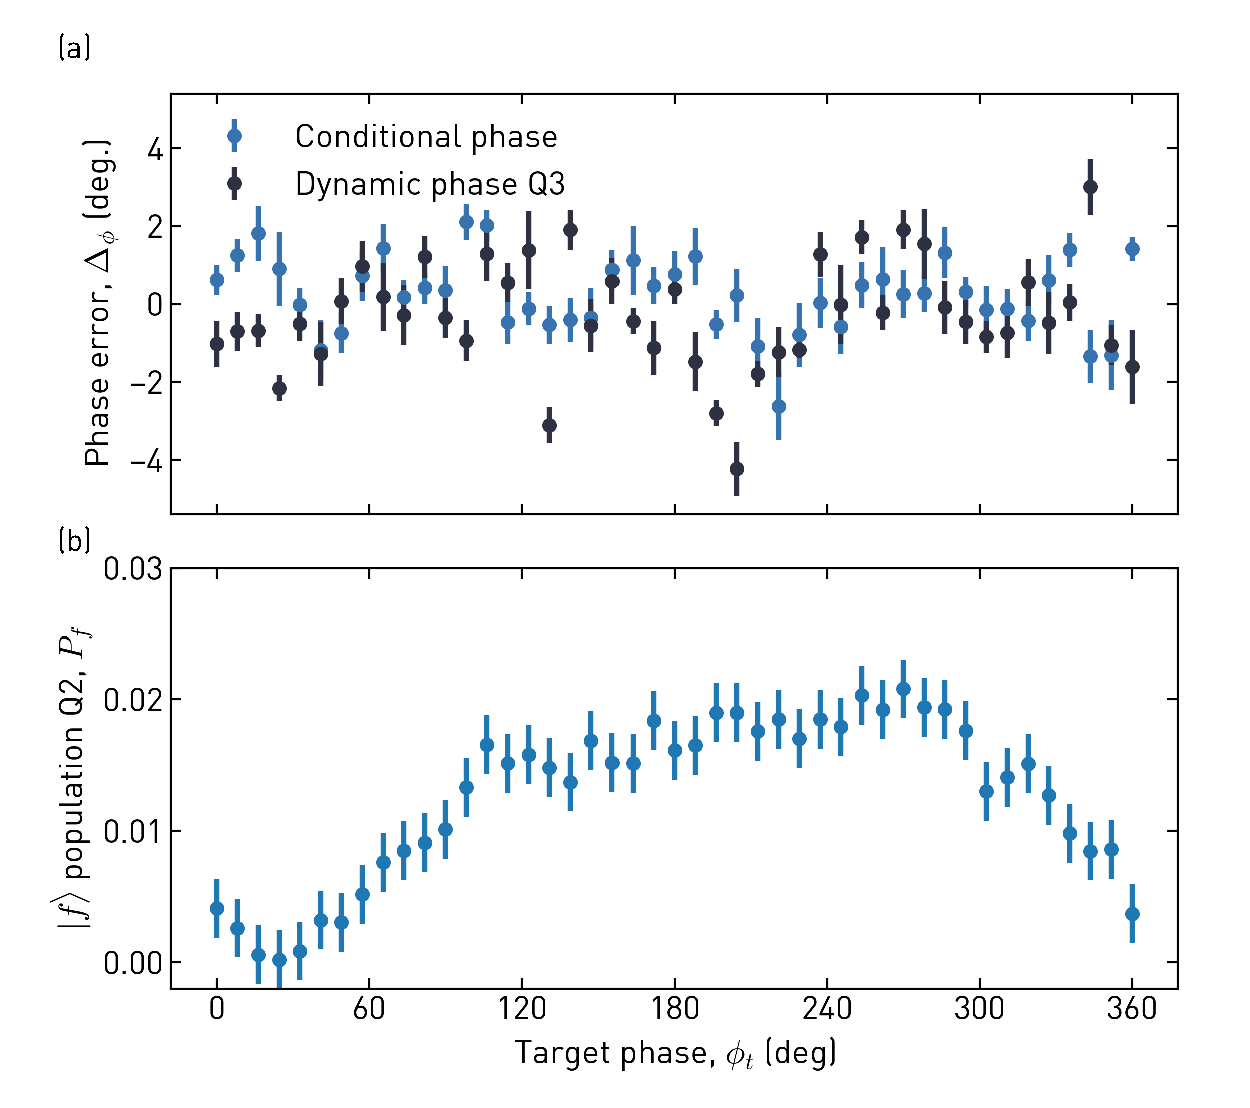
\includegraphics[width=\textwidth]{chapters/carb_gate/figs/ch4_characterization_phase_error_and_leakage_20200126_094856.pdf}
    \caption{Characterization of phase errors and leakage as function of target conditional phase with a granularity of 8\degree. Each point is averaged over 40000 single shots. (a) Conditional (light blue) and dynamic phase error (dark blue) show distributions with mean and standard distributions of $0.23\pm0.97\degree$ and  $-0.28\pm1.38\degree$ respectively. (b) We use 3-level readout to characterize leakage and measure up to 2\% leakage.}
    \label{fig:carb_characterization_phase_errors_leakage}
\end{figure}

\subsection{Comparison between C-ARB gates and CZ gates}
As final characterization procedure, we compare the \gls{carb} and \gls{cz} (implemented on the same qubits) in terms of phase errors, leakage and long term stability. We calibrate both gates and repeat the measurement described in Section~\ref{sec:carb_characterization_phase_errors_leakage}. For the \gls{cz}, we target a conditional phase of 180\degree, repeated $N$ times.  For the \gls{carb}, we sweep the range of target phases from 0 to 360\degree{} with $N$ points. These measurements are repeated for up to 15 hours after calibration. The full distributions of deviations from measured phases to target phases and leakages are presented as individual histograms, visualized as shaded filling in Fig.~\ref{fig:carb_characterization_drift}.

Both gates exhibit a similar range of conditional phase errors (standard deviation of $0.95\degree{}$ for the \gls{carb} versus $0.80\degree{}$ for the \gls{cz}). We conclude that extending the \gls{cz} to a \gls{carb} does not strongly impact the ability of preparing a target conditional phase. Note that the \gls{cz} shows a consistent offset of approximately 1\degree{} with respect to its target conditional phase. This originates from the fact that the gate is calibrated with a single point, which in this case was on the lower tail of the distribution. 

The \gls{carb} displays a wider distribution of dynamic phase errors, with an average standard deviation of 1.26\degree{} versus 0.83\degree{} for the \gls{cz}. This suggests it is harder to calibrate the dynamic phase for many flux pulse amplitudes and lengths simultaneously compared to calibrating only one. Preliminary analysis also suggest that the interpolation method has an influence on the standard deviation of the dynamic phase error. Using a cubic spline interpolation could help reduce the dynamic phase interpolation errors, compared to the implemented linear interpolation. 

The qubit 2 leakage trends are consistent with the discussion in Section~\ref{sec:carb_characterization_phase_errors_leakage}: the \gls{cz} experiences an average leakage of approximately 2\% since the \oo{} and \tz{} levels are on resonance. By contrast, the \gls{carb} experiences an average leakage of 1.4\% as several conditional phases result in low leakage. Its worse case leakage, however, is comparable to the one of the \gls{cz}. 

The phase error distributions stay relatively stable in time for both gates which suggests they will provide stable performance in algorithms for up to 15 hours after calibration.

The gates also differ in their average lengths. This effect is best visualized in Fig.~\ref{fig:ch4_calibration_carb}(a). While the \gls{cz} has a fixed flux pulse length of $107\unit{ns}$, the \gls{carb}'s flux pulse length is target phase dependent.  Averaged over all conditional phases, the flux pulse length is $84\unit{ns}$ long or $\sim 20\%$ shorter than for a conditional phase of 180 \degree. For both implementations, we add a $10\unit{ns}$ ($15\unit{ns}$) buffer at the start (end) to avoid overlap of other gates with the rising and falling edges of the flux pulse.

\begin{figure}[ht]
    \centering
    \includegraphics[width=\textwidth]{chapters/carb_gate/figs/ch4_characterization_drift_20200124_175455.png}
    \caption{Comparison between the \gls{cz} (green) and \gls{carb} (blue) in terms of phase errors and leakage as a function of time elapsed since calibration. The error bars correspond to the mean and standard deviation while the full distribution ($N$ = 45 points) is shown as shaded filling.}
    \label{fig:carb_characterization_drift}
\end{figure}

\section{Conclusion}
 In this chapter we have shown how to achieve a two-qubit unitary operation $U_{\textrm{C-ARB}}$ which adds an arbitrary phase $\phi$ on the \oo{} state. We implement this unitary by varying the frequency detuning between the \oo{} and the non-computational \tz{} state with a square,  Gaussian-filtered flux pulse. We adjust the length of the flux pulse to ensure high population recovery in the computational subspace. In practice, we calibrate the gate for a finite number of conditional phases (45) and interpolate linearly all parameters to reach phases between the calibration points. 
 
 We have characterized the gate using quantum process tomography for different conditional phases yielding a fidelity between 97.3\% and 98.3\%. The infidelity is dominated by decoherence and thermal population. In addition, we have shown that phase errors are small compared to other error mechanisms such as decoherence and residual $ZZ$-coupling. The average leakage amounts to 1.4\% and originates from the distortions of the flux pulse which are not corrected by the finite impulse response filter. The \gls{carb} shows similar time stability and phase error distributions as a \gls{cz} implemented on the same qubits while being 20\% shorter on average. 
 
 Although its calibration procedure is more elaborate, the \gls{carb} enables a significant gate count reduction for of \gls{vqa} circuits. In the next chapter, we implement a three-qubit problem instance which we solve using the \gls{qaoa} to demonstrate this advantage.


